\question[5] 
Fill in the table to give an equivalent equation in the specified form.

 \[\begin{array}{|c|c|} \hline \rule[-0.8em]{0pt}{2.2em} \textbf{Exponential Form} & \textbf{Logarithmic Form} \\ \hline \rule[-1.2em]{0pt}{3em} \hspace{3cm} & \log_{6}(P) = 2 \\ \hline \rule[-1.2em]{0pt}{3em} m = 4^{3} & \hspace{3cm} \\ \hline \rule[-1.2em]{0pt}{3em} \hspace{3cm} & \log_{2}(4) = x \\ \hline \rule[-1.2em]{0pt}{3em} e^{t} = 11 & \hspace{3cm} \\ \hline \end{array}\] 

\begin{solution}
\[\begin{array}{|c|c|} \hline \rule[-0.8em]{0pt}{2.2em} \textbf{Exponential Form} & \textbf{Logarithmic Form} \\ \hline \rule[-1.2em]{0pt}{3em} 6^{2} = P & \log_{6}(P) = 2 \\ \hline \rule[-1.2em]{0pt}{3em} m = 4^{3} & \log_{4}(m) = 3 \\ \hline \rule[-1.2em]{0pt}{3em} 2^{x} = 4 & \log_{2}(4) = x \\ \hline \rule[-1.2em]{0pt}{3em} e^{t} = 11 & \ln(11) = t \\ \hline \end{array}\]
\end{solution}


Use properties of logarithms to expand or condense the logarithmic expression as specified.
\question 
Use properties of logarithms to expand or condense the logarithmic expression as specified.\\
\begin{parts}
    \part[5] Rewrite as the sum or difference of logarithms. Express all powers as factors.

\[\log_{2}\left( \frac{8y^{3}}{4z} \right)\]

\begin{solution}
\[\log_{2}(8) + 3\log_{2}(y) - \log_{2}(4) - \log_{2}(z)\]

\[3 + 3\log_{2}(y) - 2 - \log_{2}(z)\]

\[\boxed{ 1 + 3\log_{2}(y) - \log_{2}(z) }\]
\end{solution}
    \part[5] Rewrite as a single logarithm. Express all factors as powers.

\[-\frac{1}{3}\log b + 4\log y + \log z + \log z\]

\begin{solution}
\[-\log(b^{1/3}) + \log(y^{4}) + \log(z) + \log(z)\]

\[\log\left(\frac{y^{4} z z}{\sqrt[3]{b}}\right)\]

\[\boxed{ \log\left(\frac{y^{4} z^{2}}{\sqrt[3]{b}}\right) }\]
\end{solution}
\end{parts}
\vspace{\stretch{1}}\answerline


\uplevel{For questions \ref{exact-start} through~\ref{exact-end}, solve for \textbf{all} solutions. Identify any extraneous solutions.}
\question[6] \label{exact-start}
Use the table to identify the transformations described by \(f(x) = \log_{2}(x + 1) + 1\). Circle the option that applies and fill in the blanks as appropriate to describe the transformations of the given function. If one does not apply, you may leave it blank. Then sketch the graph of the transformed function on the grid below. Indicate any asymptotes with dashed lines. 

 \[\begin{array}{|l|l|} \hline \rule[-0.8em]{0pt}{2.2em} \textbf{Horizontal Transformations} & \textbf{Vertical Transformations} \\ \hline \rule[-1.2em]{0pt}{3em} \text{Reflection: YES or NO} & \text{Reflection: YES or NO} \\ \hline \rule[-1.2em]{0pt}{3em} \text{Dilation: \underline{\hspace{2cm}} times as wide} & \text{Dilation: \underline{\hspace{2cm}} times as tall} \\ \hline \rule[-1.2em]{0pt}{3em} \text{Translation: \underline{\hspace{2cm}} units LEFT or RIGHT} & \text{Translation: \underline{\hspace{2cm}} units UP or DOWN} \\ \hline \end{array}\] 

 \[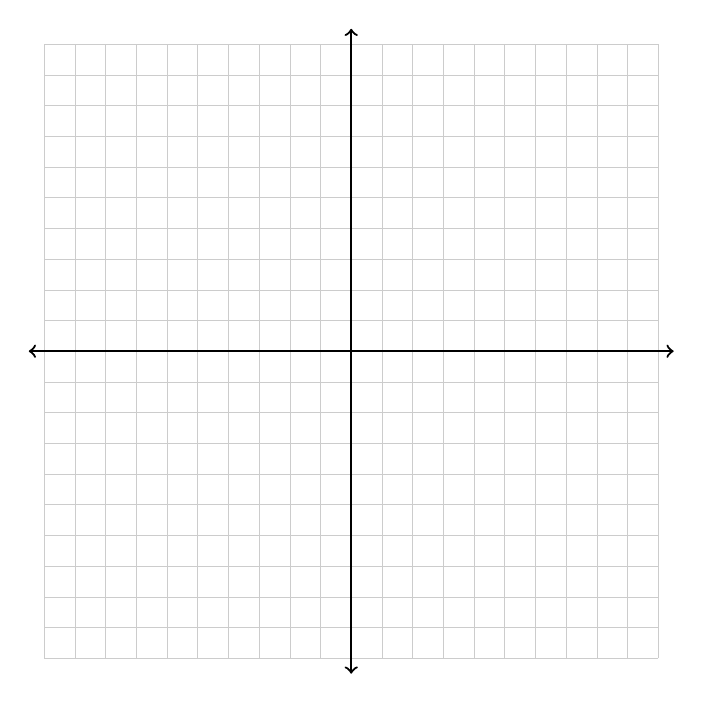
\begin{tikzpicture}[scale=0.39] \draw[step=1cm, gray!40, very thin] (-10,-10) grid (10,10); \draw[thick, <->] (-10.5,0) -- (10.5,0); \draw[thick, <->] (0,-10.5) -- (0,10.5); \end{tikzpicture}\] 

\begin{solution}
\begin{itemize}
\item
 \(\textbf{Horizontal: } \text{Reflection: NO, Dilation: 1, Shift: 1 units LEFT.}\) 

\item
 \(\textbf{Vertical: } \text{Reflection: NO, Dilation: 1, Shift: 1 units UP.}\) 

\end{itemize}


 \[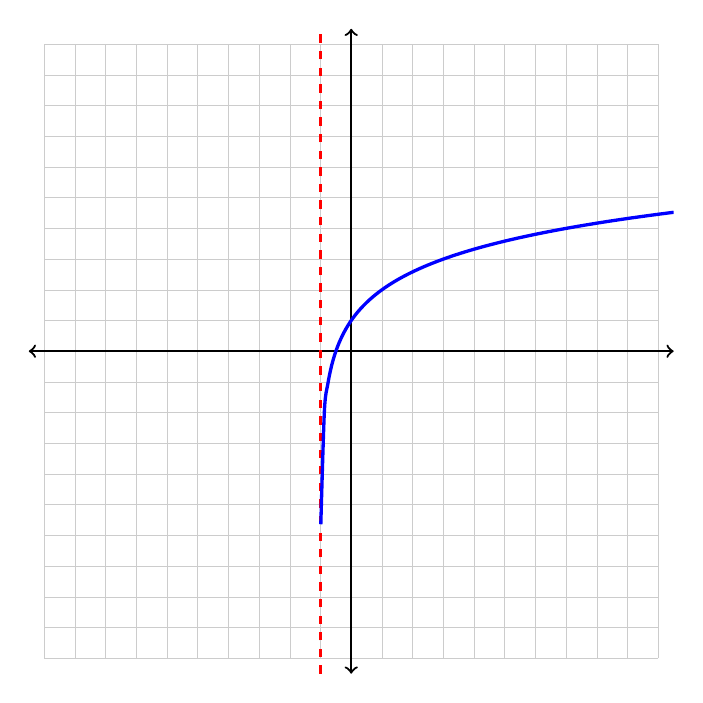
\begin{tikzpicture}[scale=0.39] \draw[step=1cm, gray!40, very thin] (-10,-10) grid (10,10); \draw[thick, <->] (-10.5,0) -- (10.5,0); \draw[thick, <->] (0,-10.5) -- (0,10.5); \clip (-10.5,-10.5) rectangle (10.5,10.5);\draw[dashed, red, thick] (-1, -10.5) -- (-1, 10.5);\draw[blue, very thick, samples=100, domain=-0.990000000000000:10.5000000000000, smooth] plot (\x, {(ln(\x - (-1))/ln(2)) + (1)});\end{tikzpicture}\]
\end{solution}
\vspace{\stretch{1}}
\par solutions: \fillin\fillin \hspace{\stretch{1}} extraneous solutions: \fillin\fillin


\question[6] 
Fill in the table below with the zeros of \(f(x) = 2 \, x^{4} + 7 \, x^{3} + 5 \, x^{2}\), their multiplicities and the behavior of the graph of the function around each zero. You may or may not use all of the rows in the table.

 \[\begin{array}{|c|c|c|} \hline \rule[-0.8em]{0pt}{2.2em} \textbf{Zero} & \textbf{Multiplicity} & \textbf{Behavior} \\ \hline \rule[-1.2em]{0pt}{3em} & & \\ \hline \rule[-1.2em]{0pt}{3em} & & \\ \hline \rule[-1.2em]{0pt}{3em} & & \\ \hline \rule[-1.2em]{0pt}{3em} & & \\ \hline \rule[-1.2em]{0pt}{3em} & & \\ \hline \end{array}\] 

\begin{solution}
\[\begin{aligned} f(x) &= 2 \, x^{4} + 7 \, x^{3} + 5 \, x^{2} \\ &= x^2(2 \, x^{2} + 7 \, x + 5) \\ &= x^2(2x + 5)(x + 1) \end{aligned}\]

 \[\begin{array}{|c|c|c|} \hline \rule[-0.8em]{0pt}{2.2em} \textbf{Zero} & \textbf{Multiplicity} & \textbf{Behavior} \\ \hline \rule[-1.2em]{0pt}{3em} -\frac{5}{2} & 1 & \text{cross} \\ \hline \rule[-1.2em]{0pt}{3em} -1 & 1 & \text{cross} \\ \hline \rule[-1.2em]{0pt}{3em} 0 & 2 & \text{bounce} \\ \hline \rule[-1.2em]{0pt}{3em} & & \\ \hline \rule[-1.2em]{0pt}{3em} & & \\ \hline \end{array}\]
\end{solution}
\vspace{\stretch{1}}
\par solutions: \fillin\fillin \hspace{\stretch{1}} extraneous solutions: \fillin\fillin

